% A Preliminary Literature Review which indicates: 
% (i) that you have studied the work of the major authors in your research field 
% (ii) that you are familiar with the major themes relevant to that subject area 
% (iii) what further investigations you intend to pursue as part of this dissertation. 
% You should bear in mind that you are reviewing the literature in order to develop sharper, 
% more insightful and focused research questions about your topic. 
% Therefore, your literature review should lead to and justify your research objectives and questions.

\xchapter{Fundamentação teórica}
{Este capítulo apresenta conceitos necessários para a compreensão do trabalho.}
\label{fundamentacao}

%À medida que os softwares se tornam uma tecnologia generalizada em praticamente
%todos os aspectos da condição humana, também são inseridos firmemente no meio
%acadêmico, softwares analisam dados, simulam o mundo real, e visualizam
%resultados.

\section{Ecossistema de software}

% ecossistema pode estar organizado em relacões de benefício mútuo

Ecossistema de software é definido, segundo \citeonline{manikas2013software},
como a interação entre diversos atores numa plataforma tecnológica comum
resultando em novas soluções de softwares ou novos serviços. Cada ator neste
sistema é motivado por um conjunto de interesses e conectam-se entre si e ao
próprio sistema numa relação simbiótica, fazendo a plataforma tecnológica
evoluir enquanto permite o envolvimento e contribuição de novos e diferentes
atores.

Nesta relação os atores são beneficiados de formas diferentes dependendo da
natureza do ecossistema, num ambiente comercial, por exemplo, os atores ganham
receita financeira diretamente (salário, prêmios, etc), enquanto num sistema
não-comercial os atores estão motivados por questões não-monetários (fama,
conhecimento, ideologia, etc).

De uma forma ou de outra, todos são beneficiados, os atores e o próprio
ecossistema, os atores recebem mais (ou melhores) benefícios com o crescimento
do ecossistema, o ecossistema oferece cada vez mais (ou melhores) benefícios
com as atividades dos seus atores, resultando numa relação de benefício
mútuo.

Este modelo geral de funcionamento do ecossistema de software pode variar a
depender do contexto em que se insere, o ecossistema de software acadêmico por
exemplo possui a particularidade de estar inserido no sistema de reputação
científica de alguma forma.

\section{Ecossistema de software acadêmico}

O ecossistema de software acadêmico possui a particularidade de estar inserido
num contexto que se relaciona com a economia de reputação científica,
especialmente com o sistema de publicação, sendo influenciado e influenciando
diretamente o impacto causado pelas suas publicações e pelo seu sistema de crédito
acadêmico.

% (5) Tools in mining software repositories \cite{chaturvedi2013tools}
% Faz uma revisão dos papers submetidos ao MSR desde 2007 até 2013 (?) e
% identifica data sets, ferramentas e técnicas utilizadas pelos autores, mais
% da metade dos papers usam ou criam ferramentas, categoriza as ferramentas em
% ferramentas novas, ferramentas tradicionais, protótipos e scripts para
% mineração de dados

\citeonline{howison2015understanding} criou um framework para pensar e refletir
sobre o processo de produção de softwares na ciência, e identificou quatro
papéis envolvidos no ecossistema de softwares acadêmicos, cientistas usuários
finais, produtores e distribuidores de software, administradores de
infraestrutura e pesquisadores preocupados com o funcionamento do ecossistema
como um todo.

\subsection{Cientistas usuários finais}

Pesquisadores de todos os domínio da ciência ocupam um papel chave no
ecossistema de software acadêmico, em seus processos de investigação e
experimentação fazem uso de artefatos de software para coletar, gerenciar,
transformar, analisar, modelar e visualizar os seus dados, sempre com o
objetivo final de publicar os seus resultados na literatura acadêmica.

Os cientistas estão preocupados com a disponibilidade, qualidade e usabilidade
destes artefatos de software e também com a capacidade de continuar úteis
podendo ser utilizados em conjunto com outros softwares. Estão interessados
também em saber o que outros cientistas usam em suas pesquisas, softwares com
alta adoção no domínio em que estão inseridos costumam manter os pesquisadores
mais livres e com maior foco em suas próprias pesquisas.

Uma alta adoção costuma ser sinal de uma boa qualidade de software, além
garantir que o grupo de pesquisa, estudantes e colaboradores consigam encontrar
mais facilmente o software e também obter ajuda entre os seus pares para
resolver questões sobre o uso do softare, simplifica também o trabalho dos
revisores pois encontrarão as mesmas facilidades no uso.

\subsection{Produtor e distribuidor de software acadêmico}

Este papel pode ser desempenhado por indivíduos ou times, softwares acadêmicos
costumam ser desenvolvidos em colaborações próximas entre cientistas da
computação e cientistas de outras áreas, usualmente sendo o cientista da
computação responsável por desenvolver algoritmos que refletem as pesquisas
destes outros pesquisadores.

Um desafio comum enfrentado pelo cientista da computação é abstrair os
problemas e implementar soluções que podem ser adotadas por outros cientistas,
especialmente em outros domínios. Alguns softwares são desenvolvidos e muitas
vezes ficam confinados em seus laboratórios ou grupos, mas eventualmente são
compartilhados e potencialmente amplamente adotados, tornando o cientista autor
do software e da pesquisa parte do ecossistema do software
\cite{howison2015understanding}.

Estes atores preocupam-se com o impacto cientifico tanto em termos de numero
quando de tipos de usuários que seu software atinge, e como seus softwares
contribuem para a ciencia que outros estão realizando.

Alguns projetos são gerenciados no estilo de código aberto, e tem atraido com
sucesso contribuições de muitos cientistas, incluindo uma calda longa de
contribuidores que tem feito pequenas mas substanciais contribuições.

\subsection{Provedor de infraestrutura}

O provedor de infraestrutura é aquele que provê um cojunto de softwares aos
cientistas usuários finais, para que dêem apoio em seus trabalhos de pesquisa.
Este conjunto de softwares podem estar disponíveis para o usuário final fazer
download eu seus computadores pessoais ou podem ser serviços de
ciberinfraestrutura de software hospedados em centros de supercomputação
usando provedores de computação em nuvem.

Do ponto de vista de ecossistema ambos os tipos de distribuição estão
interessados nas mesmas questões, quem usa ou não usa, qual versão é utilizada,
com qual frequencia atualizam, etc.

\subsection{Pesquisador}

Este último papel chamado aqui de pesquisador num sentido amplo da palavra,
refere-se à qualquer um preocupado sobre o funcionamento do próprio ecossistema
e sobre o sua contribuição para a ciência como um todo, costuma ser
desempenhado por agencias de financiamento, mas abrange qualquer cientista
preocupado com os seu trabalho individual ou do seu campo de pesquisa.

As preocupações rondam ao redor de questões sobre a operação do ecossistema como
um sistema que consome recursos (tempo, dinheiro e atenção) e afeta a conduta da
ciência, tanto no geral como em campos específicos, complementado pelo interesse
de saber como o comportamento desse sistema pode ser influenciado.

\section{Modelo de processo de softwares na ciência}

% recurso, uso e impacto

O termo ecossistema usualmente se refere a operação do sistema como um todo mas
cada ator desempenha um papel importante na estabilidade e sustentabilidade
geral do ecossistema, assim como nos ecossistemas naturais o ecossistema de
software precisa de continuas entradas (input) de energia na forma de novo
desenvolvimento ou manutenção do ecossistema \cite{dhungana2010software}.

Estes atores participam do ecossistema dentro de seus próprios interesses, mas
sempre causando um impacto de volta no sistema, os cientistas usuários finais
(direta ou indiretamente) usam softwares acadêmicos para fazer ciência,
resultando em impacto científico, este impacto científico então justifica
investimentos de novos recursos, que faz o ecossistema crescer a partir da
evolução destes softwares ou a partir da produção de novos softwares.

\begin{figure}[h]
  \center
  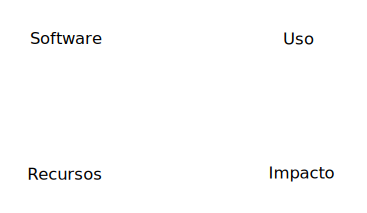
\includegraphics[scale=0.5]{imagens/process-model-scientific-software.png}
  \caption{A process model of software in science \cite{howison2015understanding}}
  \label{process-model-scientific-software}
\end{figure}

A Figura \ref{process-model-scientific-software} apresenta um diagrama deste
modelo de processo de softwares na ciência, este modelo é detalhado à seguir,
cada ator atua nos softwares, recursos, uso, impacto científico, detalhados à
seguir.

\subsection{Software}

Software acadêmico ({\it academic software}) é todo software usado para
coletar, processar ou analisar resultados de pesquisas com intenção de ser
publicados na literatura academica (seja num jornal, revista, conferência,
monografia, livro ou tese), podem ser desde protótipos escritos pelos próprios
cientistas, até mesmo produtos completos desenvolvidos profissionalmente
\cite{allen2017engineering}.

Podem ser encontrados na literatura acadêmica com outros nomes,
{\it research tool} \cite{Portillo12},
{\it research-originated software} \cite{Kon2011},
{\it research software} \cite{hettrick_2014_14809} ou
{\it scientific software} \cite{segal2008developing},
esses artefatos tem sido estudados dos mais variados pontos
de vista, desde de sua qualidade interna, até o impacto que
causam no meio científico.

No contexto de ecossistema de software acadêmico identificou-se cinco
motivações principais para a criação e contribuição ao software acadêmico:

\begin{enumerate}
  \item Ganho monetário direto (comercial software, employed software developers)
  \item Reputação acadêmica (incidental software, dirigido pela necessidade científica direta)
  \item Prática de software paralela (scientific needed enhanced by publishing 'software papers' alongside domain research)
  \item Um software de uma subárea de pesquisa (reputação direta pelo trabalho do software)
  \item Híbridos como licença-dual e 'software work' dentro de grandes colaborações (software como uma contribuição científica direta)
\end{enumerate}

\subsection{Recursos}

Os recursos investidos na produção destes softwares vem de diversas fontes,
incluem ganhos monetários diretos, recursos alocados em projetos, colaboração
entre laboratórios de pesquisa, e grande parte do ``tempo livre'' dos
pesquisadores em busca de soluções em suas pesquisas, este ``tempo livre''
perpassa por financiamentos diversos, carreira individual do cientista,
estudantes de graduação, prêmios, etc.

Independente da origem dos recursos o desenvolvimento de softwares acadêmicos
possui a particularidade de ser desenvolvido em sua grande maioria pelos
próprios cientistas uma vez que geralmente é necessário conhecimento no domínio
da pesquisa onde o software está inserido \cite{segal2008developing, hettrick_2014_14809,
momcheva2015software}.

\subsection{Uso}

% ... software é distribuido, utilizado e dá suporte à ciencia, gerando impacto ...

Estes artefatos de software são usados ativamente em diversos campos de pesquisa, como
matemática, biologia, física de partículas, astronomia, medicina e direito,
eles resolvem problemas comuns do cotidiano de pelo menos metade dos
pesquisadores de todas as áreas, desde grupos trabalhando exclusivamente com
problemas computacionais até grupos em laboratórios tradicionais ou em campo
\cite{wilson2014best}.

Os cientistas usuários finais mencionam tais softwares em suas publicações,
seja através de citação formal, informal, ou qualquer outro tipo de menção ao
software em suas pesquisas, estas citações ou menções fazem parte da economia
de reputação científica e causam impacto científico.

O impacto científico geralmente justifica o investimentos de novos recursos ao
ecossistema do software, seja para fins de planejamento, seja como
retrospectiva para avaliar os investimentos já realizados.

\subsection{Impacto científico}

% ... impacto científico justifica e potencialmente gera mais recurso ...
% \cite{katz2014transitive}

Ao longo da história, a citação formal tem sido utilizada para garantir
autenticação e autoridade, em vez de dar crédito e promover reconhecimento, na
história ocidental a citação aparece no final dos anos 1500, no início dos anos
1700 surge também no sistema legal, o ``copyright'' como reconhecendo aos
direitos autorais também surge nesse período, 1710.

A autoria das publicações tem sido realmente usado para reconhecer os autores e
contribuidores de um certo estudo, por exemplo, nos casos em que vários grupos
reivindicam crédito pelo mesmo avanço, ``backward citing'' tem sido utilizado
para verificar como as maiores comunidades de pesquisa atribuem crédito,
``forward citing'' também tem sido usada em casos onde se quer entender como
uma idéia foi usada após o seu surgimento ou publicação.

Conhecimento novo é claramente construído a partir do conhecimento passado.
Tradicionalmente, um autor cita um artigo anterior adicionando uma referência
ao autor, título, local de publicação, etc. No entanto, esse conceito não
funciona bem para produtos digitais como o software, que muitas vezes depende
de outros softwares, fragmentos de código, e algoritmos.

Este debate tem sido realizado a bastante tempo entre as diversas áreas da
bibliometria, cienciometria, altmetria e áreas similares, o fator de impacto
por exemplo proposto em 1955 apesar de continuar contribuindo para a ciência se
mostra muitas vezes utilizado da forma errada e mostra as deficiências de lidar
bem com produtos digitais gerados durante pesquisas.

\section{Sustentabilidade do ecossistema de software acadêmico}

% problemas identificados no ecossistema de software acadêmico

Um estudo sobre ecossistema de software acadêmico percebeu através dos relatos
de grande parte dos colaboradores participantes do estudo que os projetos de software
acadêmicos desenvolvidos na própria academia sofrem de {\it ``dysfunctional
chaotic churn''}, ou seja, a existência de muitos projetos, com poucos
usuários, com ciclos de vida curtos, que terminam em paralelo ao financiamento
inicial, comunidades desconectadas e paralelas, incompatibilidades entre
projetos, e tentativas aparentemente não coordenadas de ``reiniciar'' tudo
({\it re-boots}) \cite{howison2015understanding}.

Apesar de não haver evidências a respeito deste problema de forma tão abrangente,
sabe-se que parte dos problemas são realmente fato, por exemplo,
o {\it Dagstuhl Perspective Workshop}, evento organizado por um grupo de
pesquisadores sêniores de renome internacional, realizado anualmente na
universidade de Dagstuhl\footnote{\url{http://www.dagstuhl.de}} com o objetivo
refletir sobre o estado da ciência da computação explorando tópicos novos e
emergentes, em sua mais recente edição o workshop debateu sobre software
acadêmico e os problemas comuns em seu desenvolvimento, reconhecimento e
sustentabilidade \cite{allen2017engineering}.

\subsection{Desenvolvimento}

O desenvolvimento de software acadêmico ocorre em grande parte dentro da
própria academia, estudos mostram que pelo menos metade dos cientistas desenvolvem
seus próprios softwares, ao menos pacialmente, em domínios específicos este
número pode ser bem maior, na astronomia, por exemplo, estudos mostram que este
número pode chegar a 90\% \cite{hettrick_2014_14809, momcheva2015software}.

A grande participação dos cientistas no desenvolvimento destes artefatos de
software costuma ser um reflexo do tipo de conhecimento necessário ao se
desenvolver tais artefatos de software, pode ser necessário entender como o DNA
genômico se transforma em cristais de proteína, ou os meandros da dinâmica dos
fluidos, ou como resolver 20 equações diferenciais parciais simultâneas
\cite{segal2008developing}.

Desenvolvimento de software, exige algum conhecimento sobre o domínio, software
acadêmico não é diferente, mas esta grande participação dos cientistas no
desenvolvimento de software acadêmico começa a se tornar uma preocupação à
medida que a maior parte não possui treinamento algum sobre como escrever
softwares de forma eficiente, muitos não testam ou documentam os seus
softwares, faltam práticas básicas de desenvolvimento, como escrever código
legível, revisão de código, controle de versão, testes unitários, entre outros
\cite{wilson2017good}.

A qualidade dos softwares acadêmicos tem sido questionada,
a maioria também não sabe o quão confiável seu software é \cite{Merali2010Computational},
muitos estão em estado inicial de desenvolvimento \cite{marshall2013tools},
poucas foram testados fora do contexto onde foi desenvolvido \cite{Portillo12}.

Ocasionando sérios erros computacionais em conclusões centrais da literatura
acadêmica, gerando retrabalho para retratar tais erros nas mais diversas áreas
da ciência \cite{Merali2010Computational}. Dados são perdidos, análises levam
mais tempo que o necessário e os pesquisadores não conseguem a eficiência que
poderiam ter ao trabalhar com softwares acadêmicos \cite{wilson2017good}.
Causando um impacto negativo na visibilidade dos softwares acadêmicos
\cite{howison2013, katz2014transitive} e na capacidade de serem encontrados e
compartilhados.

\subsection{Reconhecimento}

% visibilidade

Apesar do crescimento no uso de software e na consequente dependência entre
cientistas de todos os campos, tornando o software acadêmico parte integral da
prática científica, apesar do apelo da comunidade científica para que o
software acadêmico seja tratado como cidadão de primeira classe, estudos tem
mostrado que muitas pesquisas não mencionam sequer o uso de software acadêmico
em suas publicações mesmo tendo feito uso de tais artefatos
\cite{momcheva2015software} \cite{howison2016software}.

Isto tem prejudicado a visibilidade do software acadêmico causando impacto
negativo em seu ecossistema, um software invisível é frequentemente excluído de
revisões por pares, uma atividade que costuma contribuir para a qualidade geral
do trabalho publicado, além disso, o
impacto negativo na visibilidade do software acadêmico faz surgir uma
série de questionamentos sobre a sua qualidade e também sobre a
capacidade de ser encontrado, compartilhado e co-desenvolvido
\cite{howison2013, katz2014transitive} \cite{howison2016software}.

Apesar de nem sempre ser possível, ou viável, ter tudo dentro de padrões
estritos, é preciso estar consciente das boas práticas ao produzir e utilizar
softwares acadêmicos, tanto para melhorar a própria abordagem quanto para
revisar outros trabalhos \cite{wilson2014best}.

Um software acadêmico em bom funcionamento devem atingir não apenas os
objetivos de entendimento e transparencia, mas também os objetivos voltados
para replicação \cite{Stodden2010}, seja logo após sua publicação, seja daqui
a 10 ou 50 anos.

\subsection{Sustentabilidade}

O desenvolvimento de software sustentável tem sido identificado como um desafio
chave no campo da ciência e da engenharia computacional, se sustentabilidade
não for levada em consideração em projetos de software, não importa qual o
domínio ou qual o propósito do software, perde-se a oportunidade de causar
mudanças positivas no planeta e na sociedade.

Apesar de sustentabilidade ser um conceito complexo e com mútiplas dimensões,
levando a debates profundos, o conceito geral é bastante simples e refe-se à
capacidade de perdurar e de continuar sendo suportado ao longo do tempo, isto
implica na qualidade de longevidade e manunetabilidade do software
\cite{venters2014software}.

Software sustentável é aquele que continua a estar disponível no futuro, em
novas plataformas, atendendo continuamente às novas necessidades do ambiente
... adequada evolução frente as condições do ambiente em constante mudança
\cite{allen2017engineering}.

Estudo mostra o decaimento das URLs ao longo do tempo, fundamenta o assunto,
mostra grafico com o caimento ao longo dos anos em publicações da
bioinformática, grafico muito bom cruzando e decaimento e tendencia com os
passar do tempo \cite{wren2017use}.

O {\it Journal of the American Statistical Association (JASA)} tem insistido na
necessiade de estarem disponíveis código e dados durante a revisão dos
manuscritos \cite{baker2016scientists}, Agências de financiamento como o {\it
US National Science Foundation} estão começando a reconhecer produtos de
pesquisa, como software, assim como fazem com as publicações, isto reconhece as
contribuições ao softwares assim como primeiro produto de pesquisa.

Isto visa especialmente garantir a longevidade dos artefatos e proporcionar que
um segundo pesquisador receba todos os benefícios do trabalho duro do primeiro
pesquisador \cite{king1995replication}, já que tanto a ciência quanto a
engenharia dependem de resultados incrementais para sua evolução. No terceiro
compromisso, relacionado ao conceito {\it desenvolvimento}, o Dagstuhl
Manifesto enfatiza a necessidade de medir a qualidade e a sustentabilidade dos
softwares científicos, tanto a priori quanto a posteriori.

\subsubsection{Manutenabilidade}

% falar de manutenabilidade como um eixo dentro de sustentabilidade técnica

A adoção e uso de softwares acadêmicos está relacionada, entre outros fatores,
também à sua qualidade, portanto é impoprtante medir e coletar sua qualidade de
alguma forma, qualidade é um vasto assunto, um dos problemas comuns enfrentado
pelos pesquisadores que desenvolvem tais softwares é a manutenabilidade
\cite{Prlic2012}.

Estudos tem mostrado que grande parte das ferramentas de software criadas na
academia estão em estado inicial de desenvolvimento \cite{marshall2013tools} e
que apenas uma pequena porcentagem são testados fora do contexto onde foi
desenvolvido \cite{Portillo12}.

%%%%%%%%%%%%%%%%%%%%%%%%%%%%%%%%%%%%%%%%%%%%%%%%%%%%%%%%%%%%%%%%%%%%%

%Cita um mapeamento feito sobre estudos que criam ferramentas para apoio a
%revisão sistemática no domínio de SE, 14 estudos foram selecionados, ao final
%apenas 8 tinham proposta de ferramentas, ao final conclui que as ferramentas
%encontradas estão em estado inicial de desenvolvimento \cite{marshall2013tools}.

%Cita um mapeamento sistemático com objetivo de encontrar ferramentas de
%comunicação e coordenação para suporte a times altamente distribuidos
%gograficamente, encontrou 132 ferramentas, para uso em projetos de software
%global. A maioria destas ferramentas foram desenvolvidas em centros de
%pesquisas, e apenas uma pequena porcentagem (18.9\%) foram testados fora do
%seu contexto onde foi desenvolvido \cite{Portillo12}.

%Computer systems research spans sub-disciplines that in-
%clude embedded and real-time systems, compilers, network-
%ing, and operating systems. Our contention is that a number
%of structural factors inhibit quality research. We highlight
%some of the factors we have encountered in our work and ob-
%served in published papers and propose solutions that could
%both increase the productivity of researchers and the quality
%of their output \cite{Vitek2011}.

%Além da aplicação, estes softwares variam também no papel que ocupam em suas
%pesquisas, alguns fazem parte dos resultados da pesquisa, como por exemplo,
%propostas de novos algoritmos ou técnicas de produção, outros são utilizados
%como parte do método de pesquisa, como coleta ou análise de dados, sendo que
%estes papeis não são excludentes.
%
%estes costumam ser citados pelos seus autores como uma das contribuições do
%estudo, seja principal ou secundária, 
%Esses softwares podem, de fato, ser um software de simulação complexo desenvolvido
%e executado em um computador de alto desempenho, mas também pode ser um
%software desenvolvido em um PC para incorporação em instrumentos; para
%manipular, analisar ou visualizar dados; ou para orquestrar fluxos de trabalho.

%e à medida
%que percebe-se que os softwares estão se tornando parte integrante dos
%processos, ferramentas e produção científicas, torna-se necessário e urgente
%discutir o seu desenvolvimento, visibilidade, qualidade e sustentabilidade.

% mostrar os beneficios da ciencia aberta, ciberinfraestrutura, etc
% * (favorecendo a ciencia e tornando a vida mais feliz para todos)

% mostrar os problemas para a ciência como um todo
% * causando problemas para o progresso de ciência, dados perdidos, etc, retrabalho
%   dificuldade de reprodução, etc...

%, não apenas técnica, mas também a
%capacidade de ser encontrado, compartilhado e co-desenvolvido, qualidades
%importantes para a evolução do próprio software, mas também extremamente útil
%para um uso eficiente dos limitados recursos da ciência \cite{howison2013,
%katz2014transitive}.

%contradizendo as boas
%práticas de qualquer projeto experimental, de ter {\it laboratory
%notebooks}\footnote{\url{https://en.wikipedia.org/wiki/Lab_notebook}}, dados
%organizados, passos documentados, e projeto estruturado para reprodutibilidade.

%softwares acadêmicos, assim
%como qualquer outro aparato experimental, são tão importantes para a ciência
%quanto são os telescópios ou tubos de ensaio \cite{wilson2014best}.

%Cientistas gastam mais tempo hoje utilizando e desenvolvendo softwares do que
%gastavam no passado.

%Software is a critical part of modern research and yet there is little support across the
%scholarly ecosystem for its acknowledgement and citation. Inspired by the activities
%of the FORCE11 working group focused on data citation, this document
%summarizes the recommendations of the FORCE11 Software Citation Working
%Group and its activities between June 2015 and April 2016. Based on a review of
%existing community practices, the goal of the working group was to produce a
%consolidated set of citation principles that may encourage broad adoption of a
%consistent policy for software citation across disciplines and venues. Our work is
%presented here as a set of software citation principles, a discussion of the motivations
%for developing the principles, reviews of existing community practice, and a
%discussion of the requirements these principles would place upon different
%stakeholders. Working examples and possible technical solutions for how these
%principles can be implemented will be discussed in a separate paper.
%\cite{smith2016software}

%Improving academic software engineering projects: A comparative study of academic and industry projects
%(compara as praticas de desenvolvimento da industria e academia e sugere melhorias, 1998!)
%https://link.springer.com/article/10.1023%2FA%3A1018925902814?LI=true

% papel pesquisador no ecossistema de soft academico
%
%Essas preocupações gerais sugerem um conjunto de questões específicas, com foco
%em padrões globais e padrões emergentes dentro do ecossistema, incluindo: Quais
%recursos foram destinados à produção de software? Quantos usuários ou
%comunidades de usuários têm projetos? Quais são os impactos científicos desse
%uso? Os números de usuários crescem? Os projetos possuem recursos e habilidades
%suficientes para gerenciar seu crescimento? Quais projetos possuem
%funcionalidades sobrepostas? Há quanto tempo os pedaços de software e projetos
%persistem? Nós desconectamos as comunidades de usuários e desenvolvedores? São
%componentes específicos, ou camadas de componentes, faltam? Que código
%geralmente é usado em conjunto; são os projetos e as pessoas que produzem esses
%componentes se comunicando adequadamente? Como podemos sustentar o software
%crítico?
%
%Aqui há uma clara tensão entre um desejo de flexibilidade e liberdade, ligado
%às expectativas de inovação científica e desejos de estruturas de autoridade e
%controle de coordenação. As questões de influência incluem: como os programas
%de financiamento e quais os requisitos em suas chamadas, resultaram em software
%amplamente utilizado e impacto científico substancial? Quais são as
%características dos campos que alcançaram maior coalescência? Quais jornais e
%conferências têm políticas exemplares? Como o trabalho de software é visto
%dentro das práticas de contratação e avaliação, como os casos de posse?
%
%\cite{howison2015understanding}

%Ao longo da história, a citação formal foi para autenticação e autoridade, em
%vez de de crédito e reconhecimento ou atribuição. A  científico citação na
%história ocidental aparece no final dos anos 1500. No início dos anos 1700, a
%citação também aparece no sistema legal como método de compreensão dos
%precedentes \cite{katz2014transitive}.

%A ideia de direitos autorais como reconhecendo aos direitos dos seus autores
%também surge nesse tempo, 1710, talvez devido a uma lenta tendência social
%societária de reconhecer a propriedade intelectual, uma idéia que parece ter se
%desenvolvido ao lado da imprensa]. Observe que a autoria de papers é realmente
%usado para notar os autores reais do artigo quanto para notar os contribuidores
%do projeto.
%Para muitos desses, o
%identificador que deve ser citado - um "nome" que se refere a um produto único
%não é claro.

%Additionally, if a cited library depends
%on another library, the contribution of this second library
%is not captured. Citation of a dataset should perhaps give
%credit to the people who gathered the data, as well as
%those who curated it, but the paper author may not know
%or be able to find these details.

%Mas independente de como seja calculado o impacto científico de uma determinada
%pesquisa o impacto causado se reverte potencialmente em mais recursos que
%poderão ser reinvestidos no próprio ecossistema onde o software está inserido.

%Science Code Manifesto \cite{barnes2013science}.
%Foco em código fonte escrito especificamente para processar dados de
%publicações, afirma que ``todo código fonte escrito especificamente para
%processar dados de uma publicação deve estar disponível para os revisores e
%leitores do paper''.

%Sustentabilidade é um conceito guarda chuva composto de múltiplas dimensões, em
%sua dimensão técnica, chamada sustentabilidade técnica, temos a preocupação com
%a longevidade da informação, dos sistemas, e infraestrutura, e sua adequada
%evolução frente as condições do ambiente em constante mudança.

%citações formais facilitam e promovem o avanço
%da ciência, mesmo diante da falta de um padrão para citar artefatos digitais
%\cite{allen2014credit}.

%Um estudo recente com 90 artigos de diversas áreas da biologia, selecionados
%aleatoriamente entre publicações usando softwares como método, mostrou que
%apenas 59 mencionavam o uso de softwares de alguma forma, os demais 31 artigos,
%apesar de usar software acadêmico, não mencionavam nada a respeito
%\cite{howison2016software}, apenas entre 31\% e 43\% das menções aos softwares
%acadêmicos envolvem citação formal.

%Não existe ainda amadurecimento suficiente sobre como citar softwares e
%outros artefatos digitais em pesquisas científicas, não temos um padrão de como fazê-lo,
%cada autor cita à sua maneira, muitas vezes ao longo do texto, outras em seções
%específicas sobre a implementação do software, nem semprem informam onde
%encontrar uma cópia do software, ou ainda nem sobre o modelo em que o software
%é distribuído, ou se é de alguma forma distribuído ao público.

%Entre os softwares acadêmicos desenvolvidos por cientistas como apoio em suas
%pesquisas, não é raro que pesquisadores deixem de disponibilizar estes artefatos,
%assim como outros desdobramentos da pesquisa, como dados e outros. Ou ainda,
%mesmo disponibilizando tais artefatos em locais de público acesso, com o tempo,
%tais locais se tornam indisponíveis inviabilizando a obtenção de tais
%artefatos.

%A comunidade tem refletido sobre os problemas relacionados ao
%desenvolvimento, promoção e sustentabilidade desses softwares, e o
%impacto que tais problemas causam no meio científico \cite{allen2017engineering}.

%, e faz
%surgir questionamentos sobre sua qualidade, não apenas técnica, mas também a
%capacidade de ser encontrado, compartilhado e co-desenvolvido, qualidades
%importantes para a evolução do próprio software, mas também extremamente úteis
%para o uso eficiente dos limitados recursos da ciência \cite{howison2013,
%katz2014transitive}.

\section{Softwares acadêmicos de análise estática} \label{analise-estatica}

Em ciência da computação, particularmente em engenharia de software, tem-se
notado um aumento constante no número de novos softwares acadêmicos
\cite{allen2017engineering}, uma área com uma longa e respeitável tradição em
pesquisas sobre a criação de novas ferramentas, métodos e algoritmos.

% (10) Analyzing the State of Static Analysis: A Large-Scale Evaluation in Open Source Software \cite{beller2016analyzing}
%
% faz um estudo mostrando que analise estatica tem uma certa adocao em projetos livres
% e mostra onde pode-se melhorar nas ferramentas para aumentar a adoção
%
% Taming the Static Analysis Beast
% \cite{toman2017taming}
% Despite advances in tooling and mainstream success, static analysis development is still a
% painful process.

\subsection{Análise estática}

A análise estática de código fonte é o primeiro passo para coletar informações
necessárias em diversas atividades de verificação, medição e melhoria da
qualidade de produtos de software \cite{Cruz2009, Kirkov2010}. Ela é
realizada com base no código fonte de um programa ou sistema de software, e a
partir daí descobre problemas e propriedades de sua qualidade estrutural
\cite{Chess2007}.

Ferramentas de análise estática estão disponíveis há décadas, em especial,
para programadores. A ferramenta Lint \cite{Johnson1978}, considerada a
primeira ferramenta de análise estática \cite{Gosain2015}, foi criada para
examinar programas escritos em linguagem C e aplicar regras de tipagem mais
estritas do que as regras dos próprios compiladores da linguagem.

Análise estática de código fonte tem como objetivo prover
informações acerca de um programa a partir do seu código fonte sem
necessidade de execução, e sem requerer qualquer outro artefato do programa
além do próprio código.

É um ramo que possui muitas das suas abordagens em comum com os estudos da
área de análise de programas ({\it program analysis}), especialmente na área de
compiladores, onde atua especialmente nas primeiras etapas do processo de compilação.

A análise estática de código fonte é considerada uma atividade meio com
objetivo de suportar uma variedade de tarefas comuns da engenharia de
software; muitas dessas tarefas são substancialmente úteis em atividades de
manutenção. \citeonline{Binkley2007} define uma lista dessas
atividades, incluindo:

\begin{multicols}{2}
  \begin{itemize}
    \item Análise de performance
    \item Compreensão de programas
    \item Desenvolvimento baseado em modelos
    \item Detecção de clones
    \item Evolução de software
    \item Garantia de qualidade
    \item Localizaçao de falhas
    \item Manutenção de software
    \item Recuperação arquitetural
    \item Testes
  \end{itemize}
\end{multicols}

Seja em qual atividade for, a análise estática possui importância,
pois ao ser capaz de extrair informações diretamente do
código fonte de um programa, pode auxiliar a responder perguntas necessárias
para as diversas atividades de desenvolvimento e evolução de software. Essa
importância se torna ainda mais aparente diante da ``lei'' da tendência para
execução \cite{Harman2010} que indica que todos os tipos de notação tem a
tendência de se tornar executáveis.

\subsection{Usos da análise estática de código fonte} \label{usos}

A análise de programas trata, de modo geral, da descoberta de problemas e
fatos sobre programas, ela pode ser realizada sem a necessidade de executar o
programa (análise estática) ou com informações provenientes de sua execução
(análise dinâmica).

A ideia de que programas de computador podem ser utilizados para analisar
código fonte de outros programas tem uma história de mais de 40 anos.  O
programa PFORT \cite{Ryder1974} foi projetado para localizar potenciais
problemas na portabilidade de código Fortran; em função da diversidade de
dialetos de Fortran, uma compilação sem erros não indicava que o programa
estava correto segundo os padrões da linguagem \cite{Wichmann1995}.

Desde então, ferramentas de análise estática de código fonte têm surgido para
os mais diversos fins -- muitas delas a partir das pesquisas e
desenvolvimentos da área de compiladores.  O {\it parser} utilizado nessas
ferramentas têm funcionalidades análogas aos analisadores usados em
compiladores \cite{Anderson2008}.

O uso de tais ferramentas tem se
tornado mais comum no ciclo de desenvolvimento de
software, sendo aplicadas em uma infinidade de atividades distintas visto que o
campo de aplicação destas ferramentas é bastante variado, cobrindo diferentes
objetivos.

%Diante a variedade e a constante evolução da área de análise estática
%\citeonline{Novak2010} fez um estudo propondo uma taxonomia e um conjunto de
%dimensões para caracterização de ferramentas de análise estática, mais detalhes
%sobre essas dimensões e categorias serão exploradas no Capítulo
%\ref{caracterizacao-ferramentas}, no qual apresentaremos uma caracterização de
%softwares científicos estudados neste trabalho.

%%%%%%%%%%%%%%%

%Neste trabalho o nosso interesse reside em compreender características de
%qualidade interna de ferramentas deste domínio de aplicação, do ponto
%de vista de desenvolvedores interessados em manter e evoluir tais ferramentas
%melhorando seus atributos de qualidade interna.
%
%A seção \ref{analise-estatica} apresenta uma definição geral da análise
%estática de código fonte, suas aplicações, sua anatomia, seus formatos de
%representação intermediária e técnicas mais comuns. 

%De acordo com \citeonline{Chess2007}, as atividades em que análise
%estática de código fonte é empregada, destacam-se:
%
%\begin{description}
%
%  \item \textit{Verificação de tipos}. 
%    A forma mais amplamente utilizada de análise estática, e uma das quais os
%    programadores estão mais familiarizados, é a checagem de tipo.
%    Previne que acidentalmente atribuam valores de forma incorreta a
%    variáveis. Ainda, ao capturar erros em tempo de compilação, esta checagem
%    de tipo previne erros em tempo de execução.
%
%  \item \textit{Verificação de estilo}. 
%    Os verificadores de estilo são um tipo de análise estática que aplicam regras
%    de forma mais superficial do que os verificadores de tipo. São regras
%    relacionadas a espaços em branco, nomes, funções depreciadas, comentários,
%    estrutura do programa, entre outros. Os erros reportados por verificadores de
%    estilo são aqueles que afetam a leitura e a manutenabilidade do
%    código fonte, não indicando potenciais erros em tempo de execução como
%    fariam os verificadores de tipo.
%
%  \item \textit{Compreensão de programas}. 
%    Ferramentas de compreensão de programa ajudam programadores a terem uma visão
%    clara frente a grandes programas de computador, ou seja, programas com
%    alto volume de código fonte. Ambientes de desenvolvimento integrados (IDE)
%    geralmente incluem funcionalidade de compreensão, por exemplo, ``encontrar
%    todos os usos de um certo método'' ou ``encontrar a declaração de uma
%    variável global''. Análises mais avançadas chegam a incluir, por exemplo,
%    refatoração automática. Estas ferramentas de compreensão também são úteis
%    para programadores interessados em entender código fonte escrito por
%    outros programadores.
%
%  \item \textit{Verificação de programas}.
%    Ferramentas de verificação de programa aceitam como entrada uma especificação
%    e um conjunto de código fonte e tenta provar que o código está deacordo
%    com a especificação. Quando a especificação é uma descrição completa de
%    todo o programa, a ferramenta de verificação poderá realizar uma checagem
%    de equivalência para garantir que o código fonte e a especificação
%    combinam de forma exata. Programadores raramente têm acesso a uma
%    especificação detalhada suficientemente para ser usada numa checagem de
%    equivalência, o trabalho de criar esta especificação pode ser maior do que
%    o trabalho de escrever o próprio código fonte do programa, desta forma
%    este tipo de verificação formal raramente acontece.
%
%  \item \textit{Localização de bugs}. 
%    Um localizador de bugs está
%    preocupado em apontar locais onde o programa, possivelmente, irá se
%    comportar de forma inesperada. A maioria das ferramentas de localização de
%    bugs são fáceis de usar porque costumam vir com um conjunto de regras
%    ({\it bug idioms}) para descrição de padrões de código que indicam bugs.
%    Algumas destas ferramentas costumam usar os mesmos algoritmos utilizados
%    por ferramentas de verificação de propriedade.
%
%  \item \textit{Avaliação de segurança}. 
%    Ferramentas de análise estática para segurança usam as mesmas técnicas
%    encontradas nas outras ferramentas, mas por ter um propósito diferente,
%    identificar problemas de segurança, aplicam estas técnicas de forma diferente.
%    As primeiras ferramentas de segurança (ITS4, RATS, Flawfinder) eram pouco mais
%    do que um {\it ``grep''} melhorado; na maior parte, elas escaneavam o código
%    procurando por funções como por exemplo {\it ``strcpy()''} que são
%    facilmente usadas de forma inadequada e devem ser inspecionadas
%    manualmente no processo de revisão de código fonte.
%
%\end{description}

%\subsection{Anatomia da análise de código fonte} \label{anatomia}
%
%Ferramentas de análise estática de código fonte estão organizadas em partes ou
%componentes, responsáveis por implementar três funções básicas: a) extração de dados, b) geração de representação
%intermediária, e c) análise \cite{Cruz2009, Binkley2007}.
%
%\begin{description}
%
%  \item \textit{Extração de dados}.
%    O processo de recuperar dados para futuro processamento ou armazenamento é
%    chamado de extração de dados. 
%
%    O primeiro componente da análise de código fonte é a extração de dados,
%    responsável por ler o código fonte do programa e gerar uma ou mais
%    representações intermediárias. Em essência, este componente converte a sintaxe
%    de um programa em uma outra sintaxe abstrata e mais adequada para análise
%    posterior.
%
%  \item \textit{Representação intermediária}.
%    Exportar os dados extraídos para uma representação intermediária é uma
%    estratégia comum para facilitar análise e transformação de dados e
%    possivelmente adição de metadados.
%
%    Os dados obtidos na extração precisam ser representados em um formato mais
%    abstrato. Esta é a responsabilidade do segundo componente da análise de
%    código fonte: armazenar os dados coletados usando uma representação
%    intermediária em formato mais adequado para análise automática, abstraindo
%    aspectos particulares do programa e da linguagem de programação.
%
%    Alguns tipos de representação intermediária têm sua origem na área de
%    compiladores, entre os formatos mais comuns, destacam-se:
%
%    \begin{multicols}{2}
%      \begin{itemize}
%        \item Árvore sintática abstrata
%        \item Grafo de fluxo de controle
%        \item Árvore sintática abstrata decorada
%        \item Grafo de dependência de módulos
%        \item Atribuição estática única
%        \item Grafo de dependência de valores
%      \end{itemize}
%    \end{multicols}
%
%    Estas representações podem ser utilizadas tanto na análise estática quanto
%    na análise dinâmica. O uso de um ou outro formato depende do tipo de
%    análise e seu propósito. Pode-se combinar diferentes tipos no sentido de
%    enriquecer e estruturar a informação extraída.
%
%  \item \textit{Análise}.
%    Este componente é responsável por realizar inferências a partir dos dados
%    representados internamente. O processo requer que as informações
%    armazenadas estejam interconectadas e também interrelacionadas com
%    conhecimento anterior. Esta análise pode gerar conhecimento quantitativo
%    ou qualitativo, como, por exemplo, métricas de software ou mineração de
%    dados, respectivamente. Técnicas de visualização podem ser usadas para
%    apoiar este processo.
%
%    Diversas técnicas foram desenvolvidas ao longo do tempo para realizar
%    análise, algumas delas são brevemente descritas na seção \ref{tecnicas}.
%
%\end{description}
%
%\subsection{Formatos de representação intermediária} \label{formatos}
%
%Essencialmente, um formato de representação intermediária é uma abstração precisa
%das propriedades de um programa representado em um domínio menor. Os
%compiladores normalmente constroem esta representação a fim de possuir um
%modelo do programa sendo compilado, é comum que compiladores utilizem diversos
%formatos durante o curso da compilação.
%
%Em ferramentas de análise estática estes formatos são utilizados durante a
%fase de análise para cumprir diversos objetivos, como por exemplo, calcular
%métricas de código fonte. A métrica de complexidade ciclomática de McCabe
%\cite{McCabe1976}, por exemplo, é definida com base no grafo de fluxo de controle ({\it Control Flow Graph - CFG}) do
%programa com o seguinte cálculo $CC = e - n + 2p$. Onde: {\bf e} é o número de
%arestas; {\bf n} é o número de nós; e {\bf p} é o número de componentes
%fortemente conectados no grafo.
%
%Assim, percebe-se que cada formato de representação intermediária pode ter fins
%e objetivos bastante distintos, dentre os formatos mais comuns podemos destacar
%\cite{Nielson2015, Stanier2013, Cruz2009, Ramalho1996}:
%
%\begin{description}
%
%  \item \textit{Árvore sintática abstrata}.
%    A árvore sintática abstrata (AST - {\it Abstract Syntax Tree}) representa um
%    programa tratando os elementos do código fonte como operadores e
%    operandos organizados em nós numa árvore, este formato de representação é
%    muito popular em tradutores {\it
%    source-to-source}\footnote{http://en.wikipedia.org/wiki/Source-to-source\_compiler}.
%
%  \item \textit{Grafo de fluxo de controle}.
%    O grafo de fluxo de controle (CFG - {\it Control Flow Graph} ou {\it Call Graph}) é um grafo direcionado
%    representando a estrutura de controle de um programa e sua sequência de
%    instruções, onde as arestas mostram os possíveis caminhos de execução. Este
%    formato é amplamente utilizado em métodos formais para otimização de
%    código fonte.
%
%  \item \textit{Grafo de fluxo de dados}.
%    O grafo de fluxo de dados (DFG - {\it Data Flow Graph}) é também um grafo
%    direcionado onde as arestas representam o fluxo de dados entre as
%    operações do programa, este formato pode ser visto como um companheiro do
%    grafo de fluxo de controle (CFG) e pode ser gerado ao longo de uma mesma
%    análise.
%
%  \item \textit{Árvore sintática abstrata decorada}.
%    Árvore sintática abstrata decorada (DAST - {\it Decorated Abstract Syntax Tree}) é
%    uma árvore sintática abstrata (AST) melhorada através de um processo de
%    definiçao de atributos para os símbolos do programa de forma declarativa
%    com uso de uma Gramática de
%    Atributos\footnote{https://en.wikipedia.org/wiki/Attribute\_grammar}.
%
%  \item \textit{Grafo de dependência de módulos}.
%    O grafo de dependência de módulos (MDG - {\it Module Dependence Graph}) é um grafo
%    onde os módulos são representados como nós e as arestas representam as
%    relacões entre eles, indicando dependência entre os mesmos.
%
%  \item \textit{Atribuição estática única}.
%    Atribuição estática única (SSA - {\it Static Single Assignment}) pode ser vista
%    como uma variação ou uma propriedade de outros formatos de representação
%    intermediária, é um método que faz cada variável ser atribuída apenas uma única
%    vez, facilitando a descoberta de informaçoes sobre os dados representados.
%
%  \item \textit{Grafo de dependência de valores}.
%    O grafo de dependência de valores (VDG - {\it Value Dependence Graph}) é uma
%    variação que melhora (ao menos para algumas análises) os resultados
%    obtidos a partir da atribuição estática única (SSA). Ele representa tanto
%    o fluxo de controle quanto o fluxo de dados e assim simplifica a análise.
%
%\end{description}
%
%\subsection{Técnicas de análise} \label{tecnicas}
%
%Inúmeras técnicas e métodos distintos podem ser utilizados pelas ferramentas
%de análise estática, seja com o objetivo de verificação de tipos, localização
%de bugs, compreensão de programas, avaliação de segurança, ou outra finalidade
%qualquer. Segundo \citeonline{German2003, Li2010, Hofer2010} as técnicas e
%métodos mais comumente encontrados nas ferramentas atuais são:
%
%\begin{description}
%
%  \item \textit{Análise léxica}.
%    A análise léxica é responsável por quebrar o programa em pequenos fragmentos
%    (ou {\it tokens}) e verificar se estes fragmentos são palavras válidas
%    para uma dada linguagem. A análise léxica não leva em consideração a
%    sintaxe do programa, sua semântica ou a interação entre módulos.
%
%  \item \textit{Combinação de padrões de texto}.
%    A combinação de padrões de texto ({\it Text-based Pattern Matching}) é a
%    maneira mais simples e rápida de procurar vulnerabilidades num código
%    fonte.
%
%  \item \textit{Inferência de tipos}.
%    A inferência de tipos ({\it Type inference}) refere-se a identificar o
%    tipo de variáveis e funções e avaliar se o acesso a elas está em
%    conformidade com as regras da linguagem. Linguagens de programação com
%    sistema de tipagem incluem mecanismos deste tipo de análise.
%
%  \item \textit{Análise de fluxo de dados}.
%    A análise de fluxo de dados ({\it Data flow analysis}) resume-se a coletar
%    informação semântica do código fonte do programa, e com métodos algébricos
%    deduzir a definição e uso das variáveis em tempo de compilação. O objetivo
%    é mostrar que nenhum caminho de execução do programa acessa uma variável
%    sem definição ou atribuição prévia.
%
%  \item \textit{Verificação de regra}.
%    A verificação de regra ({\it Rule checking}) consiste em checar a segurança
%    do programa através de um conjunto de regras pré-estabelecidas.
%
%  \item \textit{Análise de restrição}.
%    A análise de restrição ({\it Constraint analysis}) consiste em gerar
%    e resolver restrições no processo de análise de um programa.
%
%  \item \textit{Comparação caminho}.
%    Comparação caminho ({\it Patch comparison}) inclui comparação de caminho de
%    código fonte e de código-binário e é usada principalmente para encontrar
%    brechas de vulnerabilidade já ``conhecidas'' e previamente divulgadas por
%    fornecedores e praticantes da indústria de software.
%
%  \item \textit{Execução simbólica}.
%    A execução simbólica ({\it Symbolic execution}) é usada para representar
%    as entradas de um programa através do uso de valores simbólicos ao invés
%    de dados reais, produz expressões algébricas sobre a entrada dos símbolos
%    do programa durante o processo de implementação e pode detectar
%    possibilidade de erros.
%
%  \item \textit{Interpretação abstrata}.
%    Interpretação abstrata ({\it Abstract interpretation}) é uma descrição
%    formal da análise do programa. Pelo fato de apenas controlar atributos de
%    programa de preocupaçao dos usuários, a interpretação da análise semântica
%    é similar ao seu significado semântico real.
%
%  \item \textit{Prova de teoremas}.
%    Prova de teoremas ({\it Theorem proving}) é baseada na análise semântica do
%    programa. Converte o programa em fórmulas lógicas e então tenta provar que
%    o programa é um teorema válido usando regras e axiomas.
%
%  \item \textit{Verificação de modelo}.
%    O processo de verificação de modelos ({\it Model checking}) primeiro constrói
%    um modelo formal do programa tal como uma máquina de estados ou um grafo
%    direcionado, então examina e compara o modelo para verificar se o sistema
%    cumpre as características pré-definidas. Esta técnica requer a definição e
%    descrição das propriedades que devem ser verificados por um pedaço de
%    software.
%
%  \item \textit{Verificação formal}.
%    Verificação formal ({\it Formal Checking} ou {\it Compliance Analysis}) é o
%    processo de provar de forma automatizada que o código do programa está
%    correto em relação a uma especificação formal dos seus requisitos.
%
%  \item \textit{Análise de fluxo da informação}.
%    Análise de fluxo da informação ({\it Information Flow Analysis}) identifica
%    como a execução de uma unidade de código cria dependência entre entradas e
%    saídas.
%
%  \item \textit{Verificação de sintaxe}.
%    Verificação de sintaxe ({\it Syntax Checks}) tem o objetivo de encontrar
%    violação de regras tais como expressões mal-formadas ou fora do padrão.
%
%  \item \textit{Verificação de intervalo}.
%    A análise de verificação de intervalo ({\it Range Checking}) tem o objetivo
%    de verificar que os valores dos dados permanecem dentro de intervalos
%    especificados, bem como manter a precisão especificada.
%
%\end{description}


\input{capitulos/secoes/metricas.tex}
%\section{Software como cidadão de primeira classe na ciência}

JOSS, Papers executáveis, pesquisas reproduzíveis, etc, dar credibiidade ao
pesquisador cientista desenvolvedor de software ... papel do software na
reprodutibilidade, etc...

Em ciência da computação, particularmente em engenharia de software, tem-se
notado um aumento constante no número de novos softwares acadêmicos
\cite{allen2017engineering}.


%A situação com software é amplamente análoga (mas não identica) ao de dados
%das publicações; de fato, todo dado é processado por softwares de alguma forma
%(Borgman et al., 2012).

%\item The GeoScience paper of the future initiative \cite{OntoSoft2016}\footnote{\url{http://www.scientificpaperofthefuture.org/gpf/what-is-a-gpf}}
%Possui um conjunto de requerimentos para softwares serem incluidos em
%papers.  Focando mais no paper em sí do que no software.

%Linked Open Science—Communicating, Sharing and Evaluating
%Data, Methods and Results for Executable Papers.
%Linked Open Science is an approach to solve challenges of an executable paper. It is a combination of four “silver
%bullets”: 1) publication of scientific data, metadata, results, and provenance information using Linked Data principles,
%2) open source and web-based environments for executing, validating and exploring research, 3) Cloud Computing
%for efficient and distributed computing, and 4) Creative Commons for the legal infrastructure. We will use a realistic
%scientific research setting related to research on deforestation of the Brazilian Amazon rainforest to provide scenarios
%to illustrate the application of Linked Open Science \cite{Kauppinen2011}.

%Diversas maneiras de inventivar citação formal entre artefatos digitais,
%software por exemplo, tem surgido, dentre elas uma iniciativa interessante
%é o Journal of Open Source Software (JOSS) é um livre a open-access jornal para
%publicação de artigos descrevendo software acadêmico. Ele tem dois objetivos
%principais, melhorar a qualidade dos softwares submetidos e prover mecanismos
%para pesquisadores desenvolvedores de software acadêmico receber crédito pelos
%seus softwares. Enquanto pensado para trabalhar dentro do atual sistema de
%mérito da ciência, JOSS visa a escassez de recompensas para contribuições
%importantes para a ciência realizadas em forma de software. JOSS publica
%artigos que encapsulam sabedoria contida no software ele mesmo, e seu rigoroso
%revisão em pares mirado nos componentes do software: funcionalidade,
%documentação, testes, integração contínua, e a licença. Um artigo JOSS contém
%um resumo descrevendo o objetivo e funcionalidades do software, referencias, e
%um link para o software archive.  O artigo é um ponto de entrada para
%submissçao que engloba o conjunto completo de artefatos de software. Artigos
%aceitos no JOSS recebem um digital object identifier (DOI), te seus metadados
%depositados no Crossref, e o artigo pode começar a colecionar citações e ser
%indexados em serviços como Google Scholar e outros. No seu primeiro ano,
%iniciado em Maio de 2016, JOSS publicou 111 artigos, com mais de 40 artigos
%adicionais sob revisão \cite{smith2017journal}.

%\item UK RSE \cite{ukrse2013}\footnote{\url{http://rse.ac.uk/who}}
%Conscientização sobre a importância e o papel do {\it Research Software
%Engineer} através de comunicação e suporta institucional.

%FORCE11 Software Citation principles \cite{smith2016software}\footnote{\url{https://www.force11.org/software-citation-principles}}
%Enfatiza persistencia e claridade e diz que ``Software deve ser considerado
%um produto legítimo de pesquisas e devem ser possível de serem citados''.

%Reproducibility verification is essential to the practice of the scientific method.
%Researchers report their findings, which are strengthened as other independent groups
%in the scientific community share similar outcomes. In the many scientific fields
%where software has become a fundamental tool for capturing and analyzing data, this
%requirement of reproducibility implies that reliable and comprehensive software platforms
%and tools should be made available to the scientific community. The tools will empower
%them and the public to verify, through practice, the reproducibility of observations that
%are reported in the scientific literature. Medical image analysis is one of the fields in
%which the use of computational resources, both software and hardware, are an essential
%platform for performing experimental work. In this arena, the introduction of the Insight
%Toolkit (ITK) in 1999 has transformed the field and facilitates its progress by accelerating
%the rate at which algorithmic implementations are developed, tested, disseminated and
%improved. By building on the efficiency and quality of open source methodologies, ITK has
%provided the medical image community with an effective platform on which to build a daily
%workflow that incorporates the true scientific practices of reproducibility verification. This
%article describes the multiple tools, methodologies, and practices that the ITK community
%has adopted, refined, and followed during the past decade, in order to become one of the
%research communities with the most modern reproducibility verification infrastructure. For
%example, 207 contributors have created over 2400 unit tests that provide over 84% code
%line test coverage. The Insight Journal, an open publication journal associated with the
%toolkit, has seen over 360,000 publication downloads. The median normalized closeness
%centrality, a measure of knowledge flow, resulting from the distributed peer code review
%system was high, 0.46 \cite{McCormick2014}.

%Among empirical software engineering studies, those based on data re-
%trieved from development repositories (such as those of source code management,
%issue tracking or communication systems) are specially suitable for reproduction.
%However their reproducibility status can vary a lot, from easy to almost impossible
%to reproduce. This paper explores which elements can be considered to characterize
%the reproducibility of a study in this area, and how they can be analyzed to better
%understand the type of reproduction studies they enable or obstruct. One of the
%main results of this exploration is the need of a systematic approach to asses the
%reproducibility of a study, due to the complexity of the processes usually involved,
%and the many details to be taken into account. To address this need, a methodology
%for assessing the reproducibility of studies is also presented and discussed, as a tool to
%help to raise awareness about research reproducibility in this field. The application
%of the methodology in practice has shown how, even for papers aimed to be
%reproducible, a systematic analysis raises important aspects that render reproduction
%difficult or impossible. We also show how, by identifying elements and attributes
%related to reproducibility, it can be better understood which kind of reproduction
%can be done for a specific study, given the description of datasets, methodologies and
%parameters it uses \cite{gonzalez2012reproducibility}.

%Science rests on peer review and the wide-spread dissemination of
%knowledge. Software engineering research will advance further and
%faster if the sharing of data and tools were easier and more wide-
%spread. Pragmatic concerns hinder the realization of this ideal: the
%time and effort required and the risk of being scooped. We examine
%the costs and benefits of facilitating sharing in our field in an effort
%to help the community understand what problems exist and find
%a solution. We examine how other fields, such as medicine and
%physics, handle sharing, describe the value of sharing for replication
%and innovation, and address practical concerns such as standards
%and warehousing. To launch what we hope will become an ongoing
%discussion of solutions in our community, we present some ways
%forward that mitigate the risk of sharing — partial sharing, registry,
%escrow, and market \cite{barr2010shoulders}.

%At various machine learning conferences, at
%various times, there have been discussions
%arising from the inability to replicate the
%experimental results published in a paper.
%There seems to be a wide spread view that we
%need to do something to address this prob-
%lem, as it is essential to the advancement
%of our field. The most compelling argument
%would seem to be that reproducibility of ex-
%perimental results is the hallmark of science.
%Therefore, given that most of us regard ma-
%chine learning as a scientific discipline, being
%able to replicate experiments is paramount.
%I want to challenge this view by separating
%the notion of reproducibility, a generally de-
%sirable property, from replicability, its poor
%cousin. I claim there are important differ-
%ences between the two. Reproducibility re-
%quires changes; replicability avoids them. Al-
%though reproducibility is desirable, I contend
%that the impoverished version, replicability,
%is one not worth having \cite{drummond2009replicability}.

%Abstract—This paper is the result of reviewing all papers
%published in the proceedings of the former International
%Workshop on Mining Software Repositories (MSR) (2004-2006)
%and now Working Conference on MSR (2007-2009). We have
%analyzed the papers that contained any experimental analysis
%of software projects for their potentiality of being replicated.
%In this regard, three main issues have been addressed: i) the
%public availability of the data used as case study, ii) the public
%availability of the processed dataset used by researchers and iii)
%the public availability of the tools and scripts. A total number of
%171 papers have been analyzed from the six workshops/working
%conferences up to date. Results show that MSR authors use
%in general publicly available data sources, mainly from free
%software repositories, but that the amount of publicly available
%processed datasets is very low. Regarding tools and scripts, for
%a majority of papers we have not been able to find any tool,
%even for papers where the authors explicitly state that they have
%built one. Lessons learned from the experience of reviewing the
%whole MSR literature and some potential solutions to lower the
%barriers of replicability are finally presented and discussed
%\cite{robles2010replicating}.

%A survey of controlled experiments in software engineering
%Among
%the 20 replications, five can be considered as close replica-
%tions in the terminology of Lindsay and Ehrenberg [31], i.e.,
%one attempts to retain, as much as is possible, most of the
%known conditions of the original experiment.

%Replication of empirical studies in software engineering: Preliminary findings from a systematic mapping study
%The number of replications grew in the last few years, but the
%absolute number of replications is still very small, in particular
%considering the breadth of topics in software engineering. Incentive
%to perform external replications and better standards to report
%empirical studies and their replications are still needed.

%Um fator em favor da aceitação dos conceitos da EBSE tem sido a crescente
%reconhecimento que os resultados de estudos empíricos individuais são frequentemente
%inconclusivos, e estes tipo de estudos são difícels de replicar com sucesso
%\cite{sjoberg2005survey}.

%\item Reproducibility manifesto \cite{Barba2012}\footnote{\url{http://lorenabarba.com/gallery/reproducibility-pi-manifesto}}
%Inclui termos para fazer softwares reusáveis por outros. Foco em
%reprodutibilidade, deixando sustentabilidade de software fora de questão.


%mostrar os beneficios da ciencia aberta, ciberinfraestrutura, etc
%
%(favorecendo a ciencia e tornando a vida mais feliz para todos)
%
%\section{Competição no ecossistema de software acadêmico}
%
%mostrar os problemas para a ciência como um todo
%
%(causando problemas para o progresso de ciência, dados perdidos, etc, retrabalho
% dificuldade de reprodução, etc...)

%\input{capitulos/fundamentacao/qualidade-de-software.tex}
%\section{Complexidade de software}

\subsection{Manutenabilidade}

Manutenabilidade é uma característica de qualidade que indica o quão fácil é
realizar atividades de evolução e manutenção em softwares, um aspecto
importante aos pesquisadores interessados em adaptar softwares acadêmicos, algo
muitas vezes necessário ao reproduzir pesquisas anteriores \cite{Peng2011}.

%% Métricas de software podem ser classificadas em métricas de processo, métricas
%% de projeto e métricas de produto.
%% 
%% Métricas de processo medem atributos relacionados ao ciclo de desenvolvimento
%% e manutenção de software. Métricas de projeto indicam se a execução do
%% processo está progredindo conforme planejado (por exemplo, relação entre o
%% tamanho do software entregue e o esforço total dispendido em seu
%% desenvolvimento).
%% 
%% Métricas de produto medem atributos de produtos e artefatos, como documentos,
%% diagramas, código fonte e arquivos binários. Neste trabalho,
%% apenas métricas de produto serão utilizadas.
%% 
%% Métricas de produto podem ser classificadas em internas (medem propriedades
%% visíveis apenas aos desenvolvedores) ou externas (medem propriedades visíveis
%% aos usuários) \cite{Mohamed1994}.
%% 
%% Neste trabalho, são utilizadas métricas de produto e, especificamente,
%% métricas de código fonte, que cobrem aspectos de tamanho, complexidade e
%% qualidade que podem ser medidos a partir do código fonte de um software.
%% 
%% Métricas de software tem um escopo bastante abrangente, e o termo está
%% associado com muitas atividades da engenharia de software: Medidade e modelos
%% para estimativa de custo e esforço, Coleção de dados, Modelos e medidas de
%% qualidade, Modelos de confiabilidade, Métricas de segurança, Métricas
%% estruturais e de complexidade, Avaliação de maturidade de capacidade,
%% Gerenciamento através de métricas, Avaliação de métodos e ferramentas.
%% 
%% \subsection{Métricas de código fonte} \label{metricas-de-codigo}

As propriedades visíveis aos desenvolvedores podem ser medidas através de
métricas de código fonte. A observação e o monitoramento de seus valores podem
indicar aspectos relevantes à manutenibilidade de um programa. Dentre as
inúmeras métricas de código fonte nosso interesse está em métricas que indicam
características relevantes à modularidade de um produto de software,
complexidade estrutural e custo de mudança.

%Structural and Complexity Metrics
%Desirable quality attributes like reliability and maintainability cannot be
%measured until some operational version of the code is available. Yet, we
%wish to be able to predict which parts of the software system are likely to be
%less reliable, more difficult to test, or require more maintenance than oth-
%ers, even before the system is complete. As a result, we measure structural
%attributes of representations of the software that are available in advance
%of (or without the need for) execution; then, we try to establish empiri-
%cally predictive theories to support quality assurance, quality control, and
%quality prediction. These representations include control flow graphs that
%usually model code and various unified modeling language (UML) dia-
%grams that model software designs and requirements. Structural metrics
%can involve the arrangement of program modules, for example, the use
%and properties of design patterns. These models and related metrics are
%described in Chapter 9.

Do ponto de vista de métricas, neste trabalho, estamos interessados, de fato, na métrica
de complexidade estrutural SC ({\it Structural Complexity}), uma medida da
complexidade de projetos de sistema de software proposta por
\citeonline{Darcy2005} como indicador da complexidade dos sistemas de software
em relação à sua estrutura interna e ao relacionamento entre os seus
componentes.

Complexidade é um tema bastante amplo, e para compreender onde os
sistemas de softwares se encaixam neste contexto precisamos definir brevemente
o que vem a ser sistemas complexos.

Sistemas complexos são sistemas no qual grandes redes de componentes sem
controle central dão origem a um comportamento
coletivo complexo, com processamento sofisticado de informação, e adaptação
através de aprendizado ou evolução \cite{Mitchell2009}. As seguintes
características são comuns a todos os sistemas complexos:

\begin{description}

  \item[Comportamento coletivo complexo.] Apesar de serem compostos por
  elementos bastante simples individualmente, sistemas complexos podem exibir
  comportamentos coletivos bastante sofisticados.

  \item[Troca de sinais e processamento de informação.] Em cada um destes
  sistemas, seus componentes individuais consomem e produzem informação entre
  si. Parte do comportamento do sistema envolve transformação dessa informação.

  \item[Adaptação.] Sistemas complexos adaptam-se a novas situações de forma a
  aumentar suas chances de sobrevivência diante de novas condições em seu
  ambiente.

\end{description}

Os sistemas complexos podem ser classificados como naturais ou artificiais, os
sistemas naturais são aqueles cuja constituição não tem participação humana, ao
contrário dos sistemas artificiais que são projetados por humanos, com
objetivos e funções previamente definidos \cite{Simon1996}. Neste sentido,
sistemas de software podem ser caracterizados como sistemas complexos
artificiais, pois exibem comportamento coletivo complexo, realizam trocas de
sinais e processamento de informação e passam por adaptação para se adequar a
mudanças em seu ambiente.

Sistemas de software são compostos por componentes, em geral, chamados de
módulos, que possuem tanto estado quanto comportamento próprios,
módulos individuais de um sistema de software são simples quando comparados com
o sistema como um todo. Módulos produzem informação para outros módulos
através de parâmetros em chamadas de sub-rotinas e consomem informação através
dos valores de retornos destas chamadas. O fluxo contínuo de novos requisitos e
de mudanças no ambiente operacional de sistemas de software força-os a se
manter em constante evolução em busca de “sobrevivência”.

Esta medida é, possivelmente, um indicativo de problemas na manutenibilidade de
sistemas de software, em especial sobre o esforço necessário para atividades de
manutenção \cite{Terceiro2012}. Ela está relacionada a como os módulos de um
programa estão organizados bem como à estrutura interna de cada módulo. Esta
métrica pode dar indícios importantes sobre características arquiteturais de um
programa de software e pode explicar seus atributos de qualidade interna.

%Modularity
%Modularity describes the logical partitioning of software into several parts, components, and modules.
%Software will be easy to understand and change when composed of independent modules.
%“A Software Maintainability Evaluation Methodology”, 1981
%\cite{kumar2012survey}

%Faz um experimento usando CBO LCOM e outras metricas como preditor de manutenabilidade...
%\cite{Dagpinar2003}

%A complexidade de um sistema de software pode ser de três tipos: a complexidade
%do problema, a complexidade procedural, e a complexidade do projeto do sistema.
%Esta última é o foco deste trabalho.
%A complexidade do problema está relacionada ao domínio do problema.
%A complexidade procedural está relacionada à estrutura lógica da programa, em es-
%pecial do seu comprimento, em termos de número de tokens, linhas de código fonte, ou
%estruturas de controle. Este último tipo é o que iremos estudar neste trabalho.
%
%Os sistemas complexos podem naturais ou artificiais, uma colônia de formigas
%por exemplo pode ser caracterizado como um sistema complexo natural, onde
%individualmente cada formiga se apresenta como criatura relativamente simples,
%com instintos básicos como procurar alimento, responder a estímulos químicos
%vindos de outras formigas, combater intrusos, etc. No entanto, quando
%observadas coletivamente em uma colônia, as formigas aparentam ser muito mais
%sofisticadas. Elas são capazes de se organizar em diferentes atividades, criar
%estruturas complexas dentro de seu formigueiro, e de encontrar o caminho mais
%curto para uma fonte de alimento.
%
%Os sistemas naturais são aqueles cuja constituição não tem participação humana.
%Sistemas artificiais são projetados por humanos, com objetivos e funções
%definidos.  Sistemas artificiais podem ou não serem projetados à imagem de um
%sistema natural, e durante a sua concepção eles são discutidos em termos tanto
%de suas características (o que eles são) como de necessidades que eles devem
%satisfazer (o que eles deveriam ser) \cite{Simon1996}.
%
%É importante ressaltar que esta caracterização de sistemas de software como
%sistemas complexos diz respeito à estrutura interna dos sistemas, ou seja, aos
%componentes que o constituem e ao relacionamento entre estes componentes. Não
%foram considerados outros aspectos importantes de sistemas complexos, como por
%exemplo o seu relacionamento com o ambiente externo.
%
%como uma combinação das métricas de acoplamento (CBO) e coesão (LCOM4), 
%
%Sistemas de software, no entanto, se
%diferenciam dos sistemas complexos naturais pelo fato de serem projetados;
%consequentemente, o seu processo evolucionário não é intrinsecamente parte do
%seu comportamento, mas fruto da ação consciente de seus desenvolvedores.
%
%\cite{Tegarden1995}
%
%"The implication of this result is that, when
%designing, implementing, and maintaining software to control complexity, both coupling and cohesion should be considered jointly,
%instead of independently" Darcy 2005
%
%Many studies have demonstrated a significant correlation between
%LOC and the cyclomatic number. The researchers usually suggest that
%this correlation proves that cyclomatic number increases with size; that
%is, larger code is more complex code. However, careful interpretation of
%the measures and their association reveals only that the number of deci-
%sions increases with code length, a far less profound conclusion. The cyclo-
%matic number may be just another size measure. Chapter 9 contains more
%detailed discussion of validation for the McCabe measures.
%
%{\bf SC} {\it Structural Complexity (Complexidade estrutural)}: mede a
%complexidade do software \cite{Darcy2005} combinando os valores de CBO e LCOM4.

\citeonline{Darcy2005} definem complexidade estrutural como uma combinação de
acoplamento e coesão. Estes são dois conceitos complementares: enquanto o
acoplamento reflete o relacionamento entre módulos, a coesão nos fornece uma
visão da organização dos componentes internos de um módulo e seus
relacionamentos.

Uma formalização da métrica proposta por \citeonline{Darcy2005} pode ser
expressa da seguinte maneira, para um projeto $p$ e seu conjunto de módulos
$M(p)$, a complexidade estrutural $SC(p)$ de $p$ é:

\begin{equation}
SC(p) = \frac
{ \displaystyle \sum_{m \in M(p)} CBO(m) \times LCOM4(m) }
{ |M(p)| }
\end{equation}

Esta medida de complexidade estrutural é portanto a complexidade
estrutural média entre todos os módulos do sistema.

\begin{itemize}

  \item {\bf CBO} {\it Coupling Between Objects (Acoplamento entre objetos)}:
    mede o acoplamento entre objetos do software \cite{Chidamber1994}
    calculando em nível de classe o número total de acessos à outras classes do
    mesmo sistema, é comum ser também chamada de Fan-out da classe. CBO é então
    definida pela seguinte fórmula:

\begin{equation}
\label{formula-cbo}
CBO(C) = \sum_{i=1}^{n} cliente(C, Ci)
\end{equation}

Onde:

\begin{equation}
cliente(Ci, Cj) =
  \begin{cases}
    1 \text{ se } Ci \Rightarrow Cj \wedge Ci \neq Cj \\
    0 \text{ caso contrario} \\
  \end{cases}
\end{equation}

A notação $ Ci \Rightarrow Cj $ indica acesso à atributos, variáveis, métodos ou funções
entre módulos ou classes.

Apesar de ser possível formalizar a métrica CBO através da fórmula acima, sua descriçao original é
bastante complexa, levando à implementações variadas do seu cálculo
\cite{Lincke2008}. A definição original, por exemplo, inclui explicitamente
acoplamento via herança \cite{Harrison1998}, no entando não deixa claro como
deve ser tratado métodos herdados \cite{Briand1999}. A definição original
afirma também que apenas chamadas explícitas (e não chamadas implicitas) de
construtores são contabilizadas. Algumas definições de CBO incluem não apenas $
cliente(Ci, Cj) $ mas também a recíproca $ cliente(Cj, Ci) $ de forma que o valor
final inclui classes que ela acessa somado ao número de classes do sistema que
a acessam \cite{Sant2008}.

Quanto mais as classes forem independentes, mais fácil é reutilizá-las e menos
arriscado é modificá-las. Classes mais acopladas precisam de mais rigor em
testes, pois mais partes do sistema dependem delas.

  \item {\bf LCOM4} {\it Lack of Cohesion in Methods (Ausência de coesão em
    métodos)}: mede o grau de falta de coesão em métodos \cite{Hitz1995}.

O cálculo de LCOM4 é dado através de grafo não-orientado em que os nós ou
vértices são os métodos e atributos de uma classe e as arestas são acessos à
métodos e atributos. O cálculo desta métrica pode ser formalizado como a
seguir \cite{Silva2012}.

Seja $ X $ uma classe qualquer e $ M_x $ o conjunto de métodos desta classe,
considere um grafo simples não-orientado $ G_x(V, E) $, sendo:

\begin{equation}
V = M_x
\text{ e }
E = \{ \langle m, n \rangle \in V \times V \}
\end{equation}

Onde:
\begin{equation}
(\exists i \in Ix : (m \text{ accessos } i) \land (n \text{ accessos } i)) \lor (m \text{ chamadas } n) \lor (n \text{ chamadas } m)
\end{equation}

O valor da métrica LCOM4 para uma classe $ X $ é então definido como o número
de componentes conectados do grafo $ G_x (1 \leq LCOM(x) \geq | M_x |)$.

Coesão entre os métodos de uma classe é uma propriedade desejável, portanto o
valor ideal para esta métrica é 1. Se uma classe tem diferentes conjuntos de
métodos não relacionados entre si, é um indício de que a classe deveria ser
refatorada em classes menores e mais coesas.

\end{itemize}


%Isto contradiz as boas práticas de qualquer projeto experimental ({\it
%laboratory
%notebooks}\footnote{\url{https://en.wikipedia.org/wiki/Lab_notebook}}, dados
%organizados, passos documentados, projeto estruturado para reprodutibilidade) e
%torna praticamente impossível utilizar o método mais comum e cientificamente
%produtivo de produzir conhecimento novo a partir de pesquisas anteriores, a
%replicação, ou seja, seguir os mesmos passos do autor original com
%objetivo de validar, melhorar ou estender seus dados e sua metodologia
%\cite{king1995replication, Stodden2010}.

%estas práticas permitem replicar descobertas anteriores seguindo
%o caminho do autor original,
%isto, segundo
%
% Replicability is not Reproducibility: Nor is it Good Science
%
% I want to challenge this view by separating
% the notion of reproducibility, a generally de-
% sirable property, from replicability, its poor
% cousin. I claim there are important differ-
% ences between the two. Reproducibility re-
% quires changes; replicability avoids them. Al-
% though reproducibility is desirable, I contend
% that the impoverished version, replicability,
% is one not worth having.
% ...
% In this paper, I have claimed that what many in the
% field are advocating is the replicability of published
% experiments. They argue that this meets the repro-
% ducibility requirement inherent to science. My claim
% is that replicability is a poor substitute for scientific
% reproducibility. There may be other good reasons for
% the collecting of software and scripts that are the ba-
% sis of the experimental results published in papers but
% scientific reproducibility is not one.
%
%The lack of replicability and reproducibility of scientific studies based on
%computational methods has lead to serious mistakes in published scientific
%findings, some of which have been discovered and publicized recently. Many
%strategies are currently pursued to improve the situation. This article reports the
%first conclusions from the ActivePapers project, whose goal is the development
%and application of a computational platform that allows the publication of
%computational research in a form that enables installation-free deployment,
%encourages reuse, and permits the full integration of datasets and software into
%the scientific record. The main finding is that these goals can be achieved with
%existing technology, but that there is no straightforward way to adapt legacy
%software to such a framework \cite{hinsen2014activepapers}
%
%
%
%
%% Ainda existem poucos estudos replicados \cite{kitchenham2015evidence}.

% Em resumo os dois manifestos, Dagstuhl e Karlskrona, exprimem o conceito de
% sustentabilidade necessários para este estudo, mas é importante citar que
% algumas iniciativas e outros manifestos também estão preocupados com questões
% similares, dentre os quais podemos destacar:
% 
%A ciência aberta e comunidades de pesquisa em software tem sido bastante ativas
%em criar manifestos visando chamadas para ação. Estes manifestos chamam para melhorar
%os softwares e os metadados de bibliografia para citação persistente destes softwares.
%Outros tópicos endereçados nestes manifestos incluem ênfase no acesso ao código fonte.

% Software Sustainability: The Modern Tower of Babel

%Somado a isto temos ainda o fato de que pesquisadores raramente publicam seus
%códigos, piorando ainda mais toda a situação, isto tem motivado a organização
%de conferências específicas para discutir os problemas dos softwares
%acadêmicos, como o RSE (Conference of Research Software Engineers)\footnote{
%\url{http://rse.ac.uk/conf2017}}, WSSSPE (Workshop on Sustainable Software for
%Science: Practice and Experiences)\footnote{
%\url{http://wssspe.researchcomputing.org.uk}} e o RESER (Workshop on
%Replication in Empirical Software Engineering Research)\footnote{
%\url{http://sequoia.cs.byu.edu/reser}}, e tem agregado discussões das
%comunidades de ciência aberta, reprodutibilidade e sustentabilidade de
%software.

%A ciência caminha sob a teoria e experimentação \cite{vardi2010science}. Não existe ciência fechada.

%Há uma explosão de dados abertos disponíveis on-line que é acessado e analisado
%através da criação de um novo software - gerando mais dados para analisar. Os
%softwares, ou seja, qualquer software que adquira, limpe, armazene, anote,
%transforme, filtre, gere (etc.) dados de pesquisa.
